\documentclass[a4paper,11pt]{book}
%\documentclass[a4paper,twoside,11pt,titlepage]{book}
\usepackage{listings}
\usepackage[utf8]{inputenc}
\usepackage[spanish]{babel}

% \usepackage[style=list, number=none]{glossary} %
%\usepackage{titlesec}
%\usepackage{pailatino}

\decimalpoint
\usepackage{dcolumn}
\newcolumntype{.}{D{.}{\esperiod}{-1}}
\makeatletter
\addto\shorthandsspanish{\let\esperiod\es@period@code}
\makeatother


%\usepackage[chapter]{algorithm}
\RequirePackage{verbatim}
%\RequirePackage[Glenn]{fncychap}
\usepackage{fancyhdr}
\usepackage{graphicx}
\usepackage{afterpage}

\usepackage{longtable}

\usepackage[pdfborder={000}]{hyperref} %referencia

% ********************************************************************
% Re-usable information
% ********************************************************************
\newcommand{\myTitle}{Aplicación para trading algorítmico\xspace}
\newcommand{\myDegree}{Grado en ingeniería informática\xspace}
\newcommand{\myName}{Manuel Carmona Pérez\xspace}
\newcommand{\myProf}{José Manuel Benítez Sánchez\xspace}
%\newcommand{\mySupervisor}{Put name here\xspace}
\newcommand{\myFaculty}{Escuela Técnica Superior de Ingenierías Informática y de
Telecomunicación\xspace}
\newcommand{\myFacultyShort}{E.T.S. de Ingenierías Informática y de
Telecomunicación\xspace}
\newcommand{\myDepartment}{Departamento de ...\xspace}
\newcommand{\myUni}{\protect{Universidad de Granada}\xspace}
\newcommand{\myLocation}{Granada\xspace}
\newcommand{\myTime}{\today\xspace}
\newcommand{\myVersion}{Version 0.1\xspace}


\hypersetup{
pdfauthor = {\myName (email (en) ugr (punto) es)},
pdftitle = {\myTitle},
pdfsubject = {},
pdfkeywords = {palabra_clave1, palabra_clave2, palabra_clave3, ...},
pdfcreator = {LaTeX con el paquete ....},
pdfproducer = {pdflatex}
}

%\hyphenation{}


%\usepackage{doxygen/doxygen}
%\usepackage{pdfpages}
\usepackage{url}
\usepackage{colortbl,longtable}
\usepackage[stable]{footmisc}
%\usepackage{index}

%\makeindex
%\usepackage[style=long, cols=2,border=plain,toc=true,number=none]{glossary}
% \makeglossary

% Definición de comandos que me son tiles:
%\renewcommand{\indexname}{Índice alfabético}
%\renewcommand{\glossaryname}{Glosario}

\pagestyle{fancy}
\fancyhf{}
\fancyhead[LO]{\leftmark}
\fancyhead[RE]{\rightmark}
\fancyhead[RO,LE]{\textbf{\thepage}}
\renewcommand{\chaptermark}[1]{\markboth{\textbf{#1}}{}}
\renewcommand{\sectionmark}[1]{\markright{\textbf{\thesection. #1}}}

\setlength{\headheight}{1.5\headheight}

\newcommand{\HRule}{\rule{\linewidth}{0.5mm}}
%Definimos los tipos teorema, ejemplo y definición podremos usar estos tipos
%simplemente poniendo \begin{teorema} \end{teorema} ...
\newtheorem{teorema}{Teorema}[chapter]
\newtheorem{ejemplo}{Ejemplo}[chapter]
\newtheorem{definicion}{Definición}[chapter]

\definecolor{gray97}{gray}{.97}
\definecolor{gray75}{gray}{.75}
\definecolor{gray45}{gray}{.45}
\definecolor{gray30}{gray}{.94}

\lstset{ frame=Ltb,
     framerule=0.5pt,
     aboveskip=0.5cm,
     framextopmargin=3pt,
     framexbottommargin=3pt,
     framexleftmargin=0.1cm,
     framesep=0pt,
     rulesep=.4pt,
     backgroundcolor=\color{gray97},
     rulesepcolor=\color{black},
     %
     stringstyle=\ttfamily,
     showstringspaces = false,
     basicstyle=\scriptsize\ttfamily,
     commentstyle=\color{gray45},
     keywordstyle=\bfseries,
     %
     numbers=left,
     numbersep=6pt,
     numberstyle=\tiny,
     numberfirstline = false,
     breaklines=true,
   }
 
% minimizar fragmentado de listados
\lstnewenvironment{listing}[1][]
   {\lstset{#1}\pagebreak[0]}{\pagebreak[0]}

\lstdefinestyle{CodigoC}
   {
	basicstyle=\scriptsize,
	frame=single,
	language=C,
	numbers=left
   }
\lstdefinestyle{CodigoC++}
   {
	basicstyle=\small,
	frame=single,
	backgroundcolor=\color{gray30},
	language=C++,
	numbers=left
   }

 
\lstdefinestyle{Consola}
   {basicstyle=\scriptsize\bf\ttfamily,
    backgroundcolor=\color{gray30},
    frame=single,
    numbers=none
   }


\newcommand{\bigrule}{\titlerule[0.5mm]}


%Para conseguir que en las páginas en blanco no ponga cabecerass
\makeatletter
\def\clearpage{%
  \ifvmode
    \ifnum \@dbltopnum =\m@ne
      \ifdim \pagetotal <\topskip
        \hbox{}
      \fi
    \fi
  \fi
  \newpage
  \thispagestyle{empty}
  \write\m@ne{}
  \vbox{}
  \penalty -\@Mi
}
\makeatother

\usepackage{pdfpages}
\begin{document}
\begin{titlepage}
 
 
\newlength{\centeroffset}
\setlength{\centeroffset}{-0.5\oddsidemargin}
\addtolength{\centeroffset}{0.5\evensidemargin}
\thispagestyle{empty}

\noindent\hspace*{\centeroffset}\begin{minipage}{\textwidth}

\centering

\includegraphics[width=0.9\textwidth]{imagenes/logo_ugr.jpg}\\[1.4cm]

\textsc{ \Large TRABAJO FIN DE GRADO\\[0.2cm]}
\textsc{ INGENIERÍA INFORMÁTICA }\\[1cm]
% Upper part of the page
% 
% Title
{\Huge\bfseries \myTitle \\}
\noindent\rule[-1ex]{\textwidth}{3pt}\\[3.5ex]
{\large\bfseries \mySubtitle \\}
\end{minipage}

\vspace{2.5cm}
\noindent\hspace*{\centeroffset}\begin{minipage}{\textwidth}
\centering

\textbf{Autor}\\ { \myName }\\[2.5ex]
\textbf{Director}\\
{ \myProf }\\[2cm]

\includegraphics[width=0.3\textwidth]{imagenes/etsiit_logo.png}\\[0.1cm]
\textsc{\myFaculty}\\
\textsc{---}\\
Granada, mes de 2021
\end{minipage}
%\addtolength{\textwidth}{\centeroffset}
%\vspace{\stretch{2}}
\end{titlepage}



\chapter*{}
%\thispagestyle{empty}
%\cleardoublepage

%\thispagestyle{empty}

\begin{titlepage}
 
 
\setlength{\centeroffset}{-0.5\oddsidemargin}
\addtolength{\centeroffset}{0.5\evensidemargin}
\thispagestyle{empty}

\noindent\hspace*{\centeroffset}\begin{minipage}{\textwidth}

\centering
%
\includegraphics[width=0.9\textwidth]{imagenes/logo_ugr.jpg}\\[1.4cm]

%\textsc{ \Large PROYECTO FIN DE CARRERA\\[0.2cm]}
%\textsc{ INGENIERÍA EN INFORMÁTICA}\\[1cm]
% Upper part of the page
% 

 \vspace{3.3cm}

%si el proyecto tiene logo poner aquí

\includegraphics{imagenes/logo.png} 
 \vspace{0.5cm}

% Title

{\Huge\bfseries  \myTitle \\
}
\noindent\rule[-1ex]{\textwidth}{3pt}\\[3.5ex]
{\large\bfseries \mySubtitle \\[4cm]}
\end{minipage}

\vspace{2.5cm}
\noindent\hspace*{\centeroffset}\begin{minipage}{\textwidth}
\centering

\textbf{Autor}\\ { \myName }\\[2.5ex]
\textbf{Director}\\
{ \myProf }\\[2cm]
%
\includegraphics[width=0.15\textwidth]{imagenes/tstc.png}\\[0.1cm]
%\textsc{Departamento de Teoría de la Señal, Telemática y Comunicaciones}\\
%\textsc{---}\\
%Granada, mes de 201
\end{minipage}
%\addtolength{\textwidth}{\centeroffset}
\vspace{\stretch{2}}

 
\end{titlepage}






\cleardoublepage
\thispagestyle{empty}

\begin{center}
{\large\bfseries \myTitle: \mySubtitle}\\
\end{center}
\begin{center}
\myName\\
\end{center}

%\vspace{0.7cm}
\noindent{\textbf{Palabras clave}: trading algorítmico, trading automático, Wyckoff, mercados financieros}\\

\vspace{0.7cm}
\noindent{\textbf{Resumen}}\\

El volumen de datos involucrado y la velocidad a la que se realizan las operaciones de compra y venta en los mercados financieros ha hecho que la intervención de procedimientos automatizados juegue un papel fundamental en las actuales acciones de compra y venta de distintos operadores en los mercados. En estos operadores encontramos grandes inversores como entidades bancarias o instituciones.\newline

El desarrollo de algoritmos de trading es una pieza clave en la creación de estos métodos automáticos para operar. Estos algoritmos explotan técnicas de análisis de la acción de mercados financieros ya conocidas junto con métodos basados en aprendizaje automático, entre otros, para maximizar los beneficios en las compras o ventas realizadas. \newline


El objetivo de este proyecto es desarrollar una aplicación que implemente técnicas para realizar trading mediante algoritmos basados en métodos de análisis técnico ya conocidas. Esta aplicación tendrá una interfaz web para que sea usada por un operador humano.

\cleardoublepage


\thispagestyle{empty}


\begin{center}
{\large\bfseries \myTitle: \mySubtitleEnglish}\\
\end{center}
\begin{center}
Manuel Carmona Pérez\\
\end{center}

%\vspace{0.7cm}
\noindent{\textbf{Keywords}: algorithmic trading, automic trading, Wyckoff, financial markets}\\

\vspace{0.7cm}
\noindent{\textbf{Abstract}}\\

The large volume of data envolved and the speed at which the buy and sell operations are done in the financial markets have made the intervention of automated procedures a vital role in how operators buy and sell in the markets nowadays. Large investors like banks or other institutions can be found among these operators. \newline

The trading algorithms development plays a key role in these automatic methods creation. These algorithms exploit known techniques that analyze the financial markets actions and machine learning nethids, among others, to maximize benefits in the sales and purchases done. \newline

The main purpose of this project is to develop an application that implements techniques to trade by using algorithms based on already known technical analysis methods. This application will have a web interface as it will be used by a human operator.

\chapter*{}
\thispagestyle{empty}

\noindent\rule[-1ex]{\textwidth}{2pt}\\[4.5ex]

Yo, \textbf{\myName}, alumno del grado en ingeniería informática de la \textbf{Escuela Técnica Superior
de Ingenierías Informática y de Telecomunicación de la Universidad de Granada}, con DNI 17482989E, autorizo la
ubicación de la siguiente copia de mi Trabajo Fin de Grado en la biblioteca del centro para que pueda ser
consultada por las personas que lo deseen.

\vspace{6cm}

\noindent Fdo: \myName

\vspace{2cm}

\begin{flushright}
Granada, septiembre de 2021.
\end{flushright}


\chapter*{}
\thispagestyle{empty}

\noindent\rule[-1ex]{\textwidth}{2pt}\\[4.5ex]

D. \textbf{\myProf  (tutor)}, Profesor del Área de XXXX del Departamento YYYY de la Universidad de Granada.

\vspace{0.5cm}

\textbf{Informa:}

\vspace{0.5cm}

Que el presente trabajo, titulado \textit{\textbf{\myTitle, \mySubtitle}},
ha sido realizado bajo su supervisión por \textbf{\myName (alumno)}, y autorizamos la defensa de dicho trabajo ante el tribunal
que corresponda.

\vspace{0.5cm}

Y para que conste, expiden y firman el presente informe en Granada, septiembre de 2021 .

\vspace{1cm}

\textbf{Los directores:}

\vspace{5cm}

\noindent \textbf{\myProf (tutor)}

\chapter*{Agradecimientos}
\thispagestyle{empty}

       \vspace{1cm}


Poner aquí agradecimientos...


%\frontmatter
%\tableofcontents
%\listoffigures
%\listoftables
%
%\mainmatter
%\setlength{\parskip}{5pt}

%
\chapter{Introducción} \label{introduccion}

\section{Motivación}

El trading, los mercados financieros o invertir en bolsa son conceptos clásicos que hoy día están irrumpiendo más que nunca debido a los avances tecnológicos y sobre todo, gracias a la influencia de las activos digitales como las criptomonedas y otros avances de la tecnología que afectan directamente a la economía global y la centralización o no de los capitales. \newline

En este proyecto trataremos concretamente el \textit{trading} o comercio o intercambio comercial en español. El trading consiste en especular sobre distintos mercados financieros comprando o vendiendo activos para obtener un beneficio a corto o largo plazo. Estos mercados pueden ser de acciones, divisas, materias primas, índices o criptomonedas. \newline

El trading es un concepto clásico, ya que el comprar o vender algo que se puede revalorizar o devaluar para buscar beneficio económico es algo que ya se ha hecho desde las antiguas civilizaciones. En algunos documentos se habla de que la antigua civilización mesopotámica de Sumer, actual sur de Irak, fue una de las primeras en practicar el trading. Hacia el año 600 a.C., el oro y la plata ya eran las primeras monedas del mundo, antes de que se creasen los sistemas monetarios. \newline

En la actualidad, debido a la velocidad del mundo en todos los ámbitos del día a día, sobre todo en la tecnología; los procesos de compras y ventas de acciones se realizan constantemente, buscando cada operador el mayor beneficio posible y ordenando dichas operaciones a la unidad más pequeña de tiempo posible. Por esto, el trading es algo bastante avanzado y que aprovecha al máximo los recursos y conocimientos sobre la computación e inteligencia artificial actuales ya que el proceso completo se realiza de manera digital. \newline

Una de las aplicaciones de la informática en el ámbito del trading consiste en automatizar las compras y ventas de activos financieros para obtener beneficios a corto o largo plazo. Esta aplicación es la principal motivación para la realización de este trabajo de fin de grado. \newline

El objetivo principal de este \textit{Trabajo de Fin de Grado} será desarrollar una aplicación que implemente un algoritmo para automatizar el proceso de comprar y vender activos para ganar dinero. El algoritmo a implementar estará basado en la estrategia clásica para operar de \textit{Richard Wyckoff}, escritor e inversor estadounidense cofundador de \textit{The Magazine of Wall Street}. Concretamente, a esto se le conoce como trading algorítmico. En pocas palabras, el trading algorítmico es implementar un sistema de trading que opere de forma automática. \newline

	

\section{Objetivos}

El objetivo principal del proyecto es desarrollar una aplicación web para realizar trading algorítmico. El sistema implementará un algoritmo para operar basándose en técnicas de análisis de mercados financieros clásicas, en concreto, se basará en la estrategia o análisis de \textit{Richard Wyckoff}. \newline

El desarrollo principal de la aplicación se encontrará en la capacidad para comprar y vender de forma automática usando una cuenta comercial real tal y como lo haría un usuario humano, a través de un bróker o plataforma comercial de trading. Estas operaciones se realizarán según lo indique el algoritmo que elijamos, dentro de una lista de algoritmos que encontramos en la propia aplicación. \newline

La aplicación permitirá al usuario identificarse con su cuenta \textit{comercial} o \textit{demo} (de prueba) de \textit{MetaTrader5}, que será la aplicación externa que realizará las compras y ventas en el mercado financiero seleccionado. \textbf{Ref.: OBJ 1, OBJ 2.} \newline

Una vez un usuario está identificado y ha iniciado sesión en \textit{MT5}, podrá escoger un algoritmo para realizar Trading automático en tiempo real o probar las técnicas a modo de Backtesting. La aplicación también proporcionará la posibilidad de ver el histórico de operaciones realizado y el balance actual de la cuenta de \textit{MT5} en la que se ha identificado el usuario. \textbf{Ref.: OBJ 5, OBJ 6, OBJ 7, OBJ 8.} \newline

Además de poder realizar operaciones de manera automática, la aplicación dispondrá de una interfaz propia para ver los datos de mercado en tiempo real o antiguos, utilizando gráficas interactivas. \textbf{Ref.: OBJ 3, OBJ 4.}\newline

Más formalmente, podemos definir los objetivos del producto software de la siguiente forma:


\begin{itemize}
	
	\item \textbf{OBJ 1}: La aplicación tendrá un sistema de gestión de usuarios.	
	\item \textbf{OBJ 2}: El sistema conectará con la cuenta del usuario de la plataforma de trading en cuestión.
	\item \textbf{OBJ 3}: El sistema permitirá a los usuarios ver gráficos en tiempo real del mercado que se quiera visualizar.
	\item \textbf{OBJ 4}: El sistema permitirá a los usuarios ver gráficos de datos antiguos de precios del mercado que se quiera visualizar.
	\item \textbf{OBJ 5}: El sistema desarrollará varios algoritmos usados para predecir el comportamiento de los mercados y hacer compras o ventas. La aplicación permitirá a los usuarios elegir entre uno de estos algoritmos para ser usado en el resto de funciones de la APP.
	\item \textbf{OBJ 6}: El sistema permitirá a los usuarios hacer operaciones de compra y venta de manera automatizada en un periodo de tiempo y mercado concretos, eligiendo los modelos de predicción mencionados.
	\item \textbf{OBJ 7}: El sistema permitirá a los usuarios probar cada uno de los algoritmos en un periodo de tiempo fijo, a modo de backtesting.
	\item \textbf{OBJ 8}: El sistema permitirá a los usuarios ver un histórico de operaciones realizadas así como el balance actual de la cuenta a la que se ha conectado.
	
\end{itemize}


\section{Estructura del documento}

Este documento sigue la siguiente estructura de capítulos con sus respectivas secciones:\newline \\

\begin{enumerate}
	\item \textbf{Introducción}:
	Sección que incluye la motivación o justificación que lleva a la elección del tema para la elaboración del proyecto y los objetivos que se pretenden alcanzar con el mismo. 
	\item \textbf{Contexto teórico}:
	Este apartado incluye la explicación de los conceptos específicos usados a lo largo del desarrollo del proyecto. La sección habla de la teoría básica necesaria para entender ciertas decisiones y desarrollos realizados.
	\item \textbf{Planificación}: 
	Esta sección incluye cada una de las fases de la planificación temporal del proyecto, qué se ha hecho en cada fase, durante cuanto tiempo, etc. Esta planificación viene formalizada por medio de un diagrama de \textit{Gantt}. %Se incluye también en este apartado el presupuesto necesario para el desarrollo del proyecto.
	\item \textbf{Análisis}: 
	Este capítulo habla de la fase de análisis del proyecto. En esta fase se describen los implicados, los requerimientos del software a implementar y diagramas de casos de uso y comportamiento del producto.
	\item \textbf{Diseño}: 
	Este apartado incluye los principales diagramas \textit{UML} que conforman el diseño del software del proyecto. Concretamente, encontramos un diagrama de paquetes, el diseño de clases y diagramas de secuencia. Se describe también un primer diseño de la interfaz.
	\item \textbf{Implementación}: 
	En este capítulo se exponen las herramientas y software utilizado en el desarrollo del proyecto. Se habla de la metodología del trabajo, que en este caso es la metodología ágil \textit{scrum}; y del uso de issues y pull request de \textit{GitHub} y \textit{git flow}. Se describen también las fases del desarrollo y el diseño final de la interfaz.
	\item \textbf{Pruebas}: 
	Esta sección contiene la batería de pruebas realizada al producto software para comprobar su correcto funcionamiento, así como rendimiento y eficacia.
	\item \textbf{Conclusiones}: 
	En este capítulo, se describe un resumen final de lo que se ha conseguido en la realización del proyecto. En este apartado se habla de los resultados obtenidos y se expresan posibles mejoras o avances futuros.
	\item \textbf{Bibliografía}: 
	En este apartado se incluyen las referencias bibliográficas usadas a lo largo del proyecto.
	\item \textbf{Anexo}: 
	Incluye el manual de usuario de la aplicación.
\end{enumerate}
%
%\begin{titlepage}
	
\chapter{Especificación de requisitos}

\section{Objetivos}

A modo de resumen, los principales objetivos que se pretenden alcanzar con el producto software
son:

\begin{itemize}
	
	\item \textbf{OBJ 1}: El sistema conectará con la cuenta del usuario de la plataforma de trading en cuestión, para poder hacer operaciones y visualizar datos en tiempo real.
	\item \textbf{OBJ 2}: El sistema permitirá a los usuarios ver esquemas en tiempo real del mercado que se quiera visualizar.
	\item \textbf{OBJ 3}: El sistema permitirá a los usuarios hacer operaciones de compra y venta de manera manual en un mercado concreto, a través de la plataforma.
	\item \textbf{OBJ 4}: El sistema desarrollará varios modelos para predecir el comportamiento de los mercados.
	\item \textbf{OBJ 5}: El sistema permitirá a los usuarios hacer operaciones de compra y venta de manera automatizada en un periodo de tiempo y mercado concretos, eligiendo los modelos de predicción mencionados.
	\item \textbf{OBJ 6}: El sistema permitirá a los usuarios probar cada uno de los modelos en un periodo de tiempo fijo, a modo de backtesting.
	
\end{itemize}

\section{Descripción de los implicados}

En esta aplicación, destacamos dos principales implicados: el administrador de la aplicación y el usuario final de la aplicación.

\begin{itemize}
	\item \textbf{Desarrollador del sistema}: La responsabilidad del implicado será la de realizar las distintas actividades de desarrollo de la aplicación: corregir errores o añadir nuevas features, entre otras actualizaciones, que garantizan el correcto funcionamiento del sistema y su mantenimiento.
	
	\item \textbf{Usuario de la aplicación}: Este implicado representa al cliente que usa la aplicación. Este implicado hace uso de la aplicación como usuario final.
\end{itemize}

\section{Requisitos Funcionales}

Descripción de los requisitos más importantes a nivel de funciones que debe incluir el sistema, realizando una clasificación en categorías, a cada uno de los requisitos se le ha asignado un código y un nombre, con el fin de identificarlos fácilmente a lo largo de todo el proyecto. 

\begin{itemize}
	
	\item \textbf{RF-1. Gestiones de la plataforma de trading.} 
	\begin{itemize}
		\item \textbf{RF-1.1. Login en la plataforma de trading.} El usuario de la aplicación podrá conectarse con su cuenta de trading, comercial o demo, para poder hacer el uso completo de la APP.
		\item \textbf{RF-1.2. Ver capital disponible.} El usuario podrá ver el capital disponible en su cuenta de trading.
		\item \textbf{RF-1.3. El usuario podrá ver información de las operaciones} realizadas y de operaciones que en ese momento aún no se han cerrado.
	\end{itemize}

	\item \textbf{RF-2. Procesado de datos.} El usuario de la aplicación podrá proporcionar datos de mercados que procesará el sistema y que servirán de \textit{input} para cada uno de los algoritmos de predicción.

	\item \textbf{RF-3. Visualización de datos.}
	\begin{itemize}
		\item \textbf{RF-3.1. Ver datos de mercado específico.} El usuario de la aplicación podrá ver información de precios de un mercado específico.
		\item \textbf{RF-3.2. Ver datos de mercado en rango de tiempo específico.} El usuario de la aplicación podrá ver información de precios entre dos fechas específicas.
		\item \textbf{RF-3.3. Ver datos de mercado con un marco de tiempo específico.} El usuario de la aplicación podrá ver información de precios en tiempo real o entre fechas con un marco de tiempo específico.
	\end{itemize}

	\item \textbf{RF-4. El usuario podrá realizar operaciones de compra y venta de forma manual}, en un mercado, con sus respectivos parámetros.

	\item \textbf{RF-5. El usuario podrá elegir un modelo y realizar trading algorítmico.} También podrá parametrizarlo según modelo y elegir tiempo en el que quiere dejar haciendo las operaciones automáticas. 

	\item \textbf{RF-6. El usuario podrá elegir un modelo y realizar trading algorítmico a modo de backtesting.} De esta forma podrá probar cada uno de los modelos en un mercado y periodo de tiempo prefijados.
	
\end{itemize}

\section{Requisitos No Funcionales}

\begin{itemize}
	\item \textbf{RNF-1}. La plataforma de trading que usará la aplicación será MetaTrader5.
	\item \textbf{RNF-2}. La aplicación permitirá el uso de cualquier bróker aceptado por MetaTrader5, teniendo el usuario que configurar los parámetros de comisión correspondientes.
	\item \textbf{RNF-3}. Para la visualización de datos, el usuario podrá elegir un marco de tiempo de entre entre  m1, m5, m15, m30, h1, h4, d1, w1 ó mn (minutos, horas, días, semanas o meses, respectivamente).
	\item \textbf{RNF-4}. La aplicación responderá a las peticiones de los usuarios en un tiempo determinado,
	mostrando un aviso de error si el tiempo de respuesta es superior al establecido.
	\item \textbf{RNF-5}. La aplicación deberá funcionar computadoras mediante navegador web.
	\item \textbf{RNF-6}. Para la implementación de la aplicación, se utilizará Python y su framework Django.
	\item \textbf{RNF-7}. La interfaz debe ser sencilla e intuitiva.
\end{itemize}

\section{Requisitos de Información}

\begin{itemize}
	\item \textbf{RI-1}. Los datos introducidos por el usuario tendrán formato \textit{csv}. Requisitos asociados: RF-2. 
\end{itemize}

\end{titlepage}

%
%\begin{titlepage}

\chapter{Planificación}

% scrum, sprints, etc

\end{titlepage}

%
%\begin{titlepage}

\chapter{Análisis}



\end{titlepage}

%
%\begin{titlepage}

\chapter{Diseño}

% Arquitectura del software, diagramas de clases, diagramas de secuencia

\section{Arquitectura del software}

A continuación muestro un esquema equivalente a la arquitectura general del software.\newline

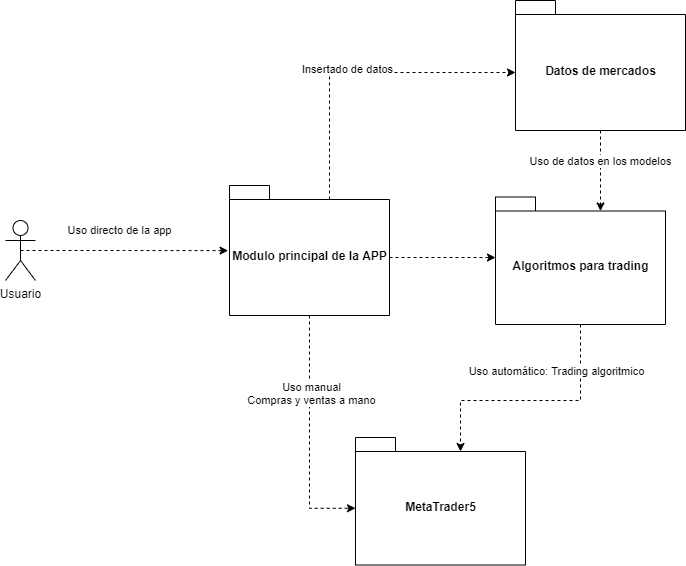
\includegraphics[width=1\textwidth]{imagenes/arquitectura general.png}\\[0.1cm]

Como resumen, en el esquema podemos ver cuál es la idea principal del proyecto. El usuario de la aplicación (véase punto 2.2, segundo implicado) será el que haga un uso directo de la interfaz de la aplicación. A continuación presento cada uno de los módulos con sus funciones y demás utilidades:\newline

\begin{itemize}
	\item \textbf{Módulo principal de la APP}: este módulo se corresponderá con el controlador principal del software. Será usado por el usuario a través de una interfaz escrita en Django y se comunicará con el resto de módulos directamente.
	\item \textbf{Datos de mercados}: este módulo se corresponderá con la base de datos y las operaciones que hagamos con dichos datos (insertado de datos, adaptaciones a cada algoritmo, etc.) Será usado por la interfaz principal de la aplicación y mandará los inputs a los algoritmos.\newline
	\item \textbf{Algoritmos para trading o backend}: se corresponde con el backend o código fuente de la aplicación. Aquí se encontrará cada uno de los algoritmos que usemos para trading algorítmico. Recibe datos de la BBDD y se comunica con el módulo de MetaTrader5 para indicar cada una de las operaciones decididas y obtener información en tiempo real.
	\item \textbf{MetaTrader5}: Módulo externo de la aplicación, se usará para mandar órdenes de operaciones y recibir resultados e información en tiempo real.
\end{itemize}

El software estará escrito en Python, usando Django como Framework para la interfaz web.
% COMPLETAR CON MAS DETALLES DE HERRAMIENTAS

\end{titlepage}
%
%\begin{titlepage}

\chapter{Implementación}



\end{titlepage}

%
%

\chapter{Pruebas}





%
%

\chapter{Conclusiones}

En este último capítulo destaco las conclusiones que podemos sacar de este trabajo de fin de grado.\newline

Divido esta sección en conclusiones de las pruebas, conclusiones de los objetivos alcanzados y futuras mejoras.\newline


\section{Conclusiones de las pruebas}

En vista de las pruebas obtenidas en el backtesting realizado en el punto anterior, podemos sacar varias conclusiones sobre la eficacia de nuestro algoritmo.\newline

El método de Wyckoff funciona de forma bastante irregular con los mercados financieros de metales y materias primas. Como hemos visto, de las pruebas realizadas en los 4 mercados: XAUUSD, XAGEUR, XBRUSD Y XNGUSD; sólo hemos obtenido un total de 9 operaciones. En otras palabras, al operar en estos mercados, la mayoría de veces mantendríamos el algoritmo funcionando sin que ordene operaciones de compra y venta. Este comportamiento puede deberse a la estabilidad quizás de dichos mercados financieros. Si comparamos estos mercados con los intercambios de divisas, tenemos mercados menos populares y que eso al final, afecta directamente al comportamiento de los precios. \newline

Si un mercado es poco popular entre los operadores, esto supondrá spreads altos, ya que tendremos menos gente que compre al precio que piden los que venden. Spread alto indica menos liquidez. Ver punto 2 de la memoria, contexto teórico del proyecto. \newline

Esto puede ser una justificación de que las operaciones sean malas en dichos mercados. Pero realmente lo que ocurre es que no se ordenan operaciones. \newline

¿A qué puede deberse esto? Bien, la implementación del algoritmo de detección de tendencias, usado en el método de Wyckoff, usaba Bandas de Bollinger. Si volvemos al apartado de implementación, veremos que las Bandas de Bollinger son una medida de volatilidad del precio. Cuando tenemos tendencias bajistas y alcistas, hay más volatilidad en el mercado y es justo con esto con lo que tratamos en el algoritmo. ¿Qué ocurre en el caso de los mercados mencionados, que tienen más spread? Siempre habrá poca volatilidad. Es por esto que nuestro algoritmo tenderá a no encontrar tendencias como lo haría en divisas, donde hay más volatilidad.\newline


Finalmente hablo de los resultados de la ejecución del método de Wyckoff en el mercado de divisas, EURUSD.\newline

En este caso, obtenemos relativamente buenos resultados. En Min15 obtenemos resultados positivos, en H1 también. En la temporalidad de H4, cada 4 horas, hemos obtenido una pérdida; y en D1 hemos obtenido ganancias.\newline

De aquí podemos sacar una conclusión clara, que tiene que ver con la gestión de riesgo. ¿Qué está ocurriendo en Min15 y H1 que no pasa en H4? Estamos aplicando más de una operación, mientras que en H4, sólo realizamos una. Aquí, como he dicho, entra en juego la gestión de riesgo. Cuando definimos el método de Wyckoff, describimos que para ordenar una operacion, el take profit, o valor en el que cerrábamos en ganancias la operación, debería de suponer el doble de ganancias que el stop lose, o valor en el que cerramos con pérdidas. Esto, a efectos teóricos, implica que si hemos realizado dos operaciones; una de ellas beneficiosa y otra con pérdidas; habremos obtenido ganancias en el recuento general.\newline

Por esto, si en H4 se hubiese hecho alguna operación más, tendríamos quizás ganancias, debido a la gestión de riesgo mencionada.\newline

Hablando de nuevo en general de todos los resultados de todos los mercados, no podemos mirar el balance como un número. Este balance debe ser visto como un acierto o una ganancia. ¿Por qué? A la hora de operar en la vida real, los operadores utilizan el lotaje para realizar las inversiones. El lotaje o lote, a efectos prácticos sería el tanto por ciento de activo que compras al invertir. Si compras más lote, tu balance final será el obtenido en estas presuntas situaciones por un multiplicador.\newline

En el caso de la última prueba realizada durante 4 años en la divisa EURUSD en H1 (mencionado al final del capítulo anterior), aunque las ganancias sean pocas, si controlamos el número de lotes, podríamos obtener grandes beneficios. \newline

Como conclusión final, el algoritmo resultante es bueno para operar con EURUSD u otras divisas. Con posibles mejoras, el algoritmo podría ser perfectamente usado por un operador humano en una operativa en tiempo real. En cuanto al resto de mercados financieros, no parece un algoritmo adecuado debido a los problemas antes mencionados. \newline

\section{Objetivos alcanzados}

En la introducción de esta memoria, se hablaba de una serie de objetivos propuestos en el proyecto. En esta sección estudiamos cada uno de ellos y si se ha realizado correctamente o no.\newline

Se han completado todos los objetivos propuestos al inicio del trabajo:

\begin{itemize}
	\item Se ha implementado el sistema de gestión de usuarios
	\item Se ha implementado la conexión con el bróker y plataforma de trading MT5.
	\item Se ha implementado la funcionalidad de ver gráficos en tiempo real del mercado que se quiera visualizar a cualquier marco de tiempo.
	\item Se ha implementado la funcionalidad de ver gráficos de datos antiguos, recogidos de una base de datos previamente guardada por el usuario, de forma automática.
	\item Se ha implementado la estrategia o método de Wyckoff para trading algorítmico.
	\item Se permite a los usuarios realizar operaciones de compra y venta de manera automatizada seleccionando algoritmo.
	\item Se permite a los usuarios realizar backtesting, a modo de prueba de algoritmos.
	\item Se permite a los usuarios ver las operaciones realizadas y balance.
\end{itemize}

También podemos destacar, que el desarrollo del sistema para trading algorítmico cumple con las ventajas expuestas en el apartado de trading algorítmico:

\begin{itemize}
	\item Diversificación: cumplimos con dicha ventaja. A pesar de la menor eficacia en los mercados financieros mencionados, el algoritmo puede ser usado para todos los mercados financieros. Como mencioné en dicha ventaja, existe la posibilidad de que en ciertos mercados obtengamos beneficios con una técnica que no obtenemos con otra.
	\item Evaluación de técnicas: se puede realizar una evaluación numérica de los resultados obtenidos.
	\item Evitamos las emociones.
	\item Podemos desplegar el proyecto en la nube. En este caso, podríamos montar un servidor con Windows que levantase el proyecto y conectarnos a él via internet.
\end{itemize}

\section{Futuras mejoras}

En esta sección propongo posibles futuras mejoras de la aplicación.\newline

Como se ha propuesto en anteriores apartados, mejorar el método de Wyckoff podría ser una posible mejora. En este punto cabría destacar la creación de nuevos análisis de otro tipo de diagramas que Wyckoff expuso en sus enfoques, como bien podría ser el de Punto y Figura. Gracias a estos nuevos análisis, controlaríamos mejor los volúmenes de precios y ofera/demanda, esfuerzo/resultado, etc.\newline

Otra mejora o ampliación sería la inclusión y estudio de nuevos métodos. Esto es sencillo ya que por construcción, la aplicación permite el desarrollo y uso de nuevos algoritmos.\newline

También se podría cambiar o mejorar el sistema de gestión de datos, para poder guardar datos de distintos mercados simultáneamente. Actualmente sólo se permite un mercado con una temporalidad al mismo tiempo. En este punto entraría también la posibilidad de realizar un guardado de dichos datos en la nube.\newline
%
%%\chapter{Conclusiones y Trabajos Futuros}
%
%
%%\nocite{*}
%\bibliography{bibliografia/bibliografia}\addcontentsline{toc}{chapter}{Bibliografía}
%\bibliographystyle{miunsrturl}
%
%\appendix
%\input{apendices/manual_usuario/manual_usuario}
%%\input{apendices/paper/paper}
%\input{glosario/entradas_glosario}
% \addcontentsline{toc}{chapter}{Glosario}
% \printglossary
\chapter*{}
\thispagestyle{empty}

\end{document}
